% TEX compiler = luatex
% copyright arturo salinas-aguayo 2025
\documentclass[12pt]{article}

\usepackage{graphicx}
\usepackage{subcaption}
\usepackage{amsmath}
\usepackage{array}
\usepackage{amsfonts}
\usepackage{fancyhdr}
\usepackage{geometry}
\usepackage{circuitikz}
\usepackage{caption}
\usepackage{karnaugh-map}
\usepackage{bm}
\usepackage{float}

\geometry{letterpaper, margin=1in}
\graphicspath{ {../../images/} }

% Header and Footer
\pagestyle{fancy}
\fancyhf{}
\fancyhead[L]{ECE 2001 - Lab 06: Passive Filter Circuits}
\fancyhead[R]{\thepage}
\setlength{\headheight}{15pt}

\author{Arturo Salinas-Aguayo}
\title{Lab 006: Passive Filter Circuits}

% theorem set
\newtheorem{example}{Example}
% Example block environment
\newenvironment{examp}
{\vspace{0.5cm}
 \hrule
\vspace{0.5cm}
\begin{example}}
{\hrule
\vspace{0.5cm}
\end{example}}

\begin{document}
\newcommand{\closure}[2][3]{%
	{}\mkern#1mu\overline{\mkern-#1mu#2}}
\newcommand\ncoverline[1]{\mkern1mu\overline{\mkern-1mu#1\mkern-1mu}\mkern1mu}
% Title Page
\begin{titlepage}
	\centering
	\vspace*{3cm}
	\huge\textbf{Lab 06: Passive Filter Circuits}\\

	\vspace{5cm}
	\Large\textbf{Arturo Salinas-Aguayo}\\
	\normalsize
	ECE 2001 Electrical Circuits\\
	Dr. David J. Giblin, Section 331.660.701.810-1253\\
	Mechanical Engineering Department
	\vfill
	
\includegraphics[scale=0.1]{uconnlogo}\\
	College of Engineering, University of Connecticut\\
	\scriptsize{Coded in \LaTeX}
	\vspace*{1cm}
\end{titlepage}
\tableofcontents
\newpage
\section{Abstract}
Passive filters have a wide variety of applications such as within dc power
supplies to eliminate unwanted high-frequency noise within the ac-line or in
radios to provide the listener with only the desired signal while rejecting all
other unwanted signals. They also work on the transmission side, allowing only a
certain signal to be generated while attenuating the others that might cause
interference.

Another, perhaps more relevant application is that off a crossover
network in which a passive filter is used to adjust the audio signals going to
speakers to properly balance audio between tweeters, woofers, and midrange
speakers. This lab introduces these concepts and expands upon the knowledge
gained in learning about inductors and capacitors, while leaving things such as
alternating current sources still unexplained. For this reason, this
experimental work will focus on the frequency response and phase shift
characteristics of these filters rather than the analysis of the circuits in
theory.

\newpage
\section{Introduction}

While earlier labs focused on transient response, this experiment shifts attention to the steady-state sinusoidal behavior of electrical filters. The objective is to analyze how the amplitude and phase of a circuit’s output vary with input frequency. By constructing and testing first-order and second-order filters, this lab builds intuition for practical applications in audio electronics, communication systems, and signal processing.

Filters are circuits that selectively permit certain frequency components while rejecting others. A low-pass filter allows low-frequency signals to pass while attenuating higher frequencies. Conversely, a high-pass filter does the opposite, blocking low frequencies and allowing high-frequency signals through. The critical threshold between the passband and stopband is the \textit{cutoff frequency}, typically defined as the point where the output amplitude falls to $\frac{1}{\sqrt{2}}$ (approximately 0.707) of the input signal, corresponding to a $-3\,\mathrm{dB}$ gain relative to the passband.

Second-order filters, such as the RLC bandpass filter studied in this lab,
exhibit more complex behavior including resonance, which is especially relevant
in tuned circuits used in radios, amplifiers, and frequency-selective networks.


\section{Theory}
\subsection{A Quick Introduction to Filters}
Filters are circuits which are purposefully designed to allow certain and reject
others. Passive filters are studied in this experimental work which are
constructed with resistors, capacitors, and inductors. At this point, the study
of the frequency domain has been just introduced, so the math will not get too
heavy just yet. However, utilizing SPICE simulation, the frequency response of
circuits can be obtained and modeled accurately.

\subsection{Low-Pass RC Filter}

A first-order RC low-pass filter consists of a resistor in series with the input and a capacitor to ground at the output. This configuration allows low-frequency signals to charge the capacitor, which then appears as an open circuit to DC, while higher frequencies are shorted to ground through the capacitor’s decreasing reactance.

The transfer function of the low-pass RC filter is:
\[
	H(f) = \frac{1}{1 + j2\pi fRC}
\]
The magnitude of this function decreases as frequency increases. The cutoff frequency, where the gain drops by $3\,\mathrm{dB}$, is given by:
\[
	f_c = \frac{1}{2\pi RC}
\]

\subsection{High-Pass RC Filter}

A high-pass filter is formed by swapping the positions of the resistor and capacitor. In this configuration, the capacitor initially blocks low-frequency signals (including DC), but its reactance decreases with frequency, allowing higher-frequency components to pass through more easily.

The transfer function becomes:
\[
	H(f) = \frac{j2\pi fRC}{1 + j2\pi fRC}
\]
With the same cutoff frequency:
\[
	f_c = \frac{1}{2\pi RC}
\]
At very low frequencies, the gain approaches zero; at very high frequencies, the gain approaches unity.

\subsection{Second-Order RLC Circuit (Bandpass Filter)}

A second-order series RLC circuit includes a resistor, inductor, and capacitor in series. When driven by a sinusoidal source, the circuit exhibits a resonance at a specific frequency where the inductive and capacitive reactances cancel each other out. At this frequency, the impedance is minimized (equal to $R$), and the output voltage across the resistor is maximized.

The resonance (or natural) frequency is:
\[
	f_0 = \frac{1}{2\pi\sqrt{LC}}
\]
The sharpness of the resonance peak is characterized by the \textit{quality factor}, $Q$, defined as:
\[
	Q = \frac{1}{R} \sqrt{\frac{L}{C}}
\]

Higher $Q$ values correspond to narrower, more selective bandpass responses (underdamped), while lower $Q$ values lead to broader frequency responses (overdamped). The bandwidth of the filter is inversely proportional to $Q$ and directly affected by the resistance in the circuit.

\section{Experimental Procedures}

\subsection{Circuit One: RC High-Pass Filter}
This circuit forms a basic first-order high-pass filter. The output is taken across the resistor. A $22\,\mathrm{nF}$ capacitor was used in place of the originally specified $15\,\mathrm{nF}$ to better match desired cutoff behavior. The schematic is shown in Figure~\ref{fig:circuitone}.

\begin{figure}[H]
	\centering
	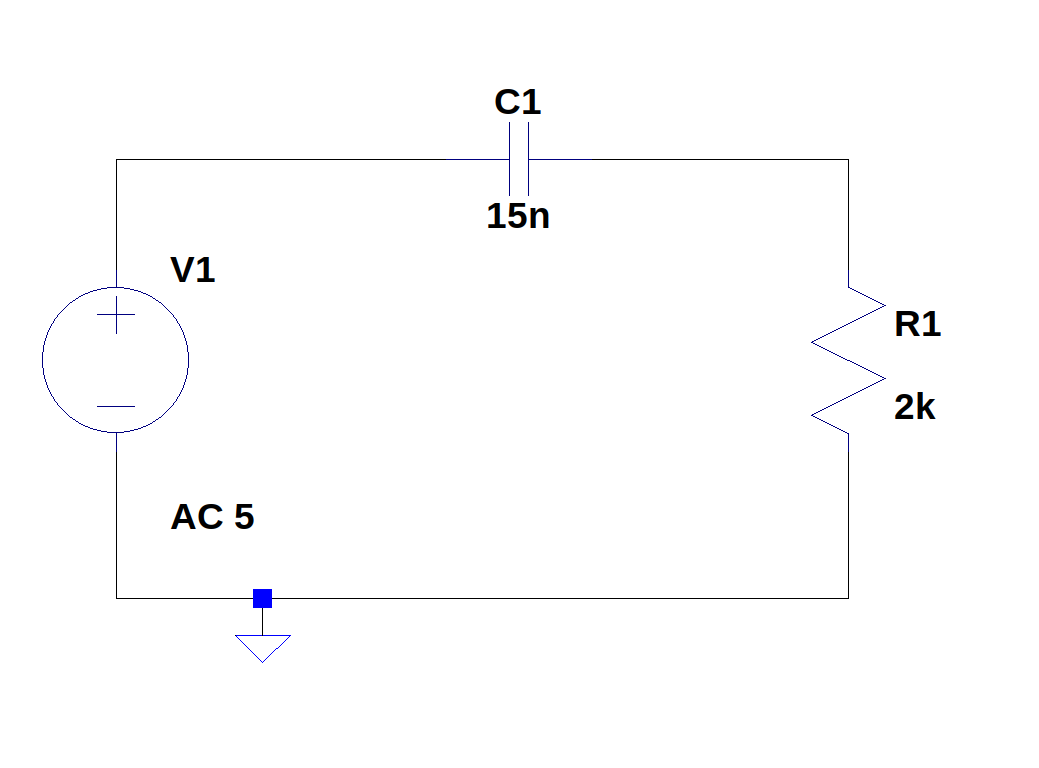
\includegraphics[width=0.5\textwidth]{e6_01}
	\caption{Circuit One – RC High-Pass Filter (Output Across Resistor)}
	\label{fig:circuitone}
\end{figure}

\noindent \textbf{Measured Values:}
\begin{itemize}
	\item Cutoff Frequency: $3556.31\,\mathrm{Hz}$
	\item Phase at Cutoff: $45.49^\circ$
\end{itemize}

\subsection{Circuit Two: RC Low-Pass Filter}
This low-pass configuration is identical in components to Circuit One, but the output is instead taken across the capacitor. The resulting filter allows lower frequencies to pass while attenuating higher ones. The schematic is shown in Figure~\ref{fig:circuittwo}.

\begin{figure}[H]
	\centering
	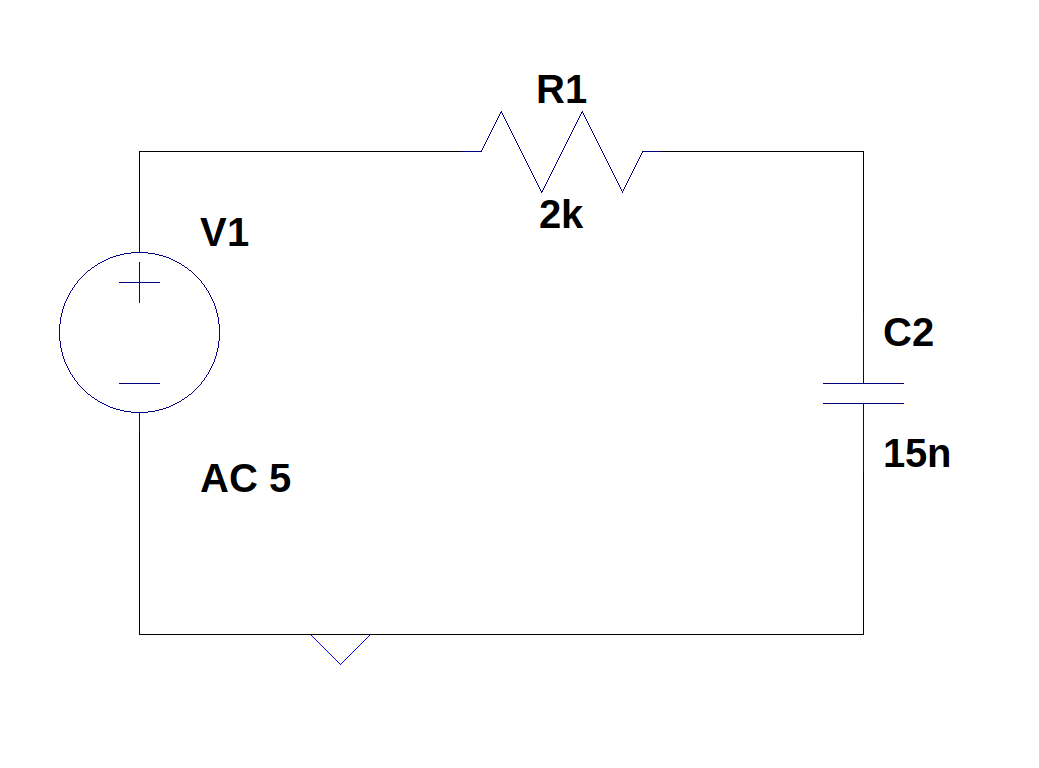
\includegraphics[width=0.5\textwidth]{e6_02}
	\caption{Circuit Two – RC Low-Pass Filter (Output Across Capacitor)}
	\label{fig:circuittwo}
\end{figure}

\noindent \textbf{Measured Values:}
\begin{itemize}
	\item Cutoff Frequency: $3681.29\,\mathrm{Hz}$
	\item Phase at Cutoff: $-45.50^\circ$
\end{itemize}

\subsection{Circuit Three: Parallel Capacitor Low-Pass Filter}
Circuit Three builds on the previous configurations by adding a second capacitor in parallel. This increases the filter's order and steepens the roll-off in the stopband. The circuit schematic is provided in Figure~\ref{fig:circuitthree}.

\begin{figure}[H]
	\centering
	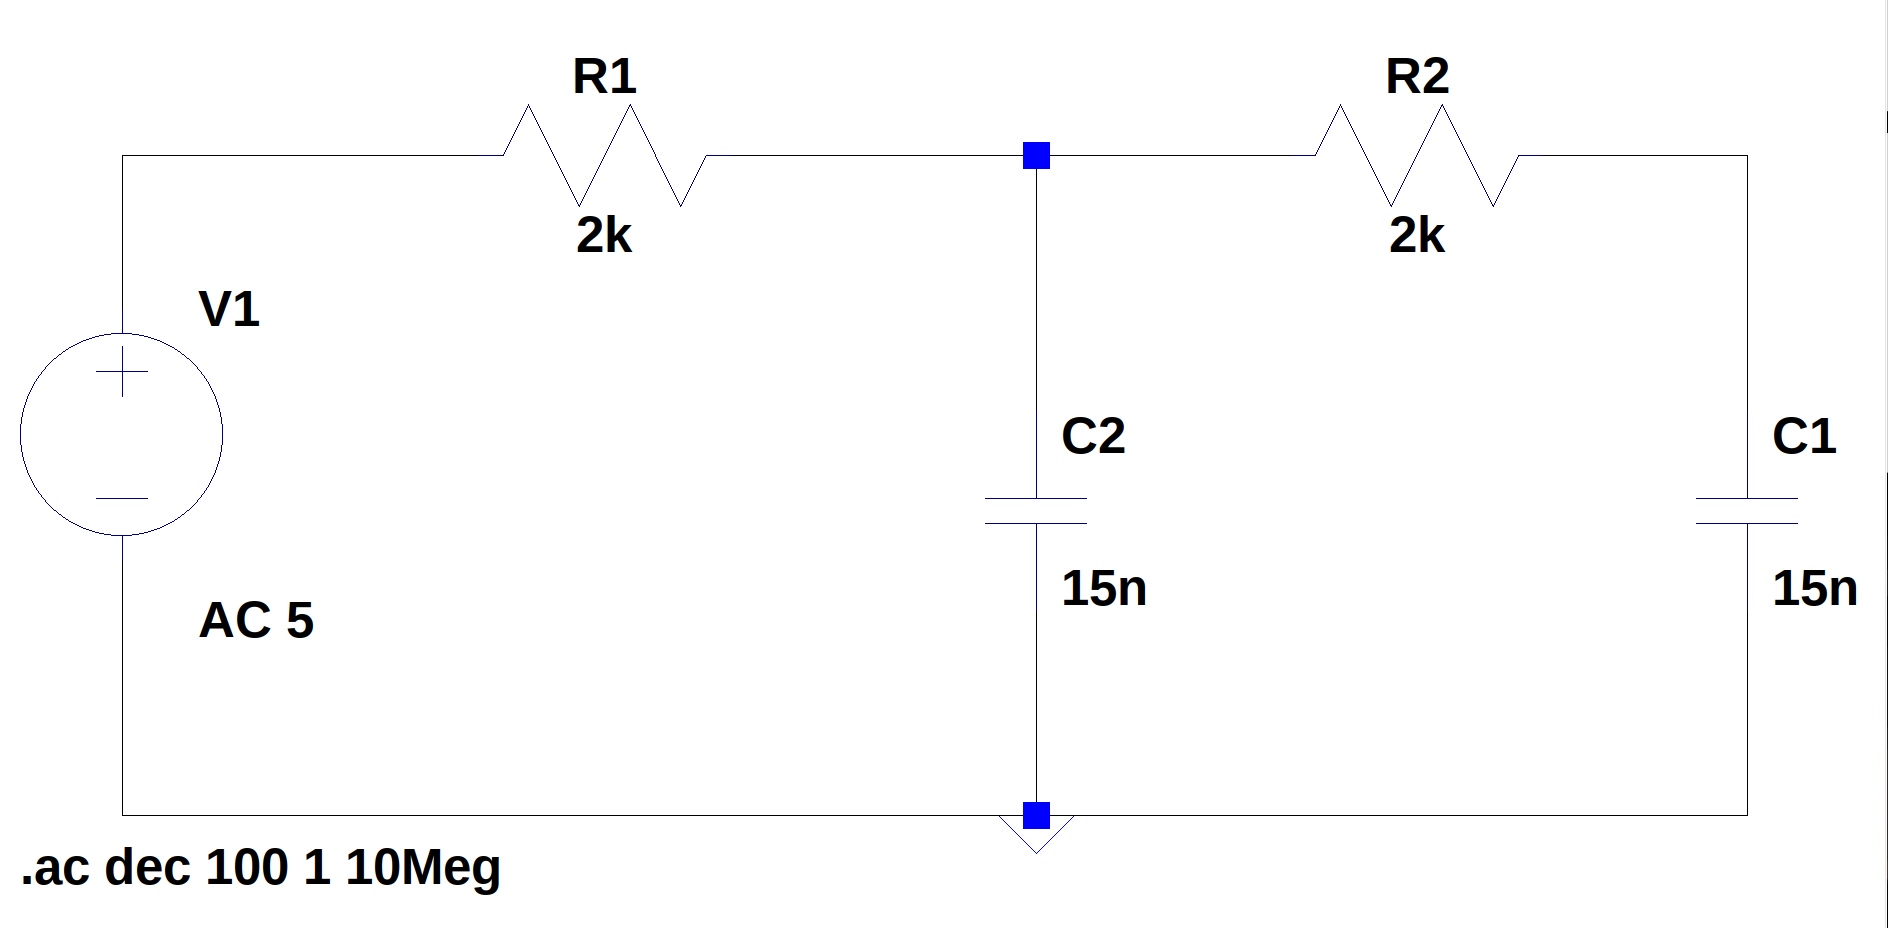
\includegraphics[width=0.5\textwidth]{e6_03}
	\caption{Circuit Three – Second-Order RC Low-Pass Filter}
	\label{fig:circuitthree}
\end{figure}

\noindent \textbf{Measured Values:}
\begin{itemize}
	\item Cutoff Frequency: $1377.21\,\mathrm{Hz}$
	\item Phase at Cutoff: $-53.18^\circ$
\end{itemize}

\subsection{Circuit Four: Series RLC Bandpass Filter}
Circuit Four introduces an inductor to create a second-order RLC bandpass filter. This configuration allows a narrow range of frequencies to pass while attenuating both low and high frequencies. Two versions were tested: one with a low resistance ($200\,\Omega$) and another with high resistance ($2000\,\Omega$), to compare underdamped and overdamped behavior.

\subsubsection*{Case 1: $R = 200\,\Omega$ (Underdamped)}
\begin{figure}[H]
	\centering
	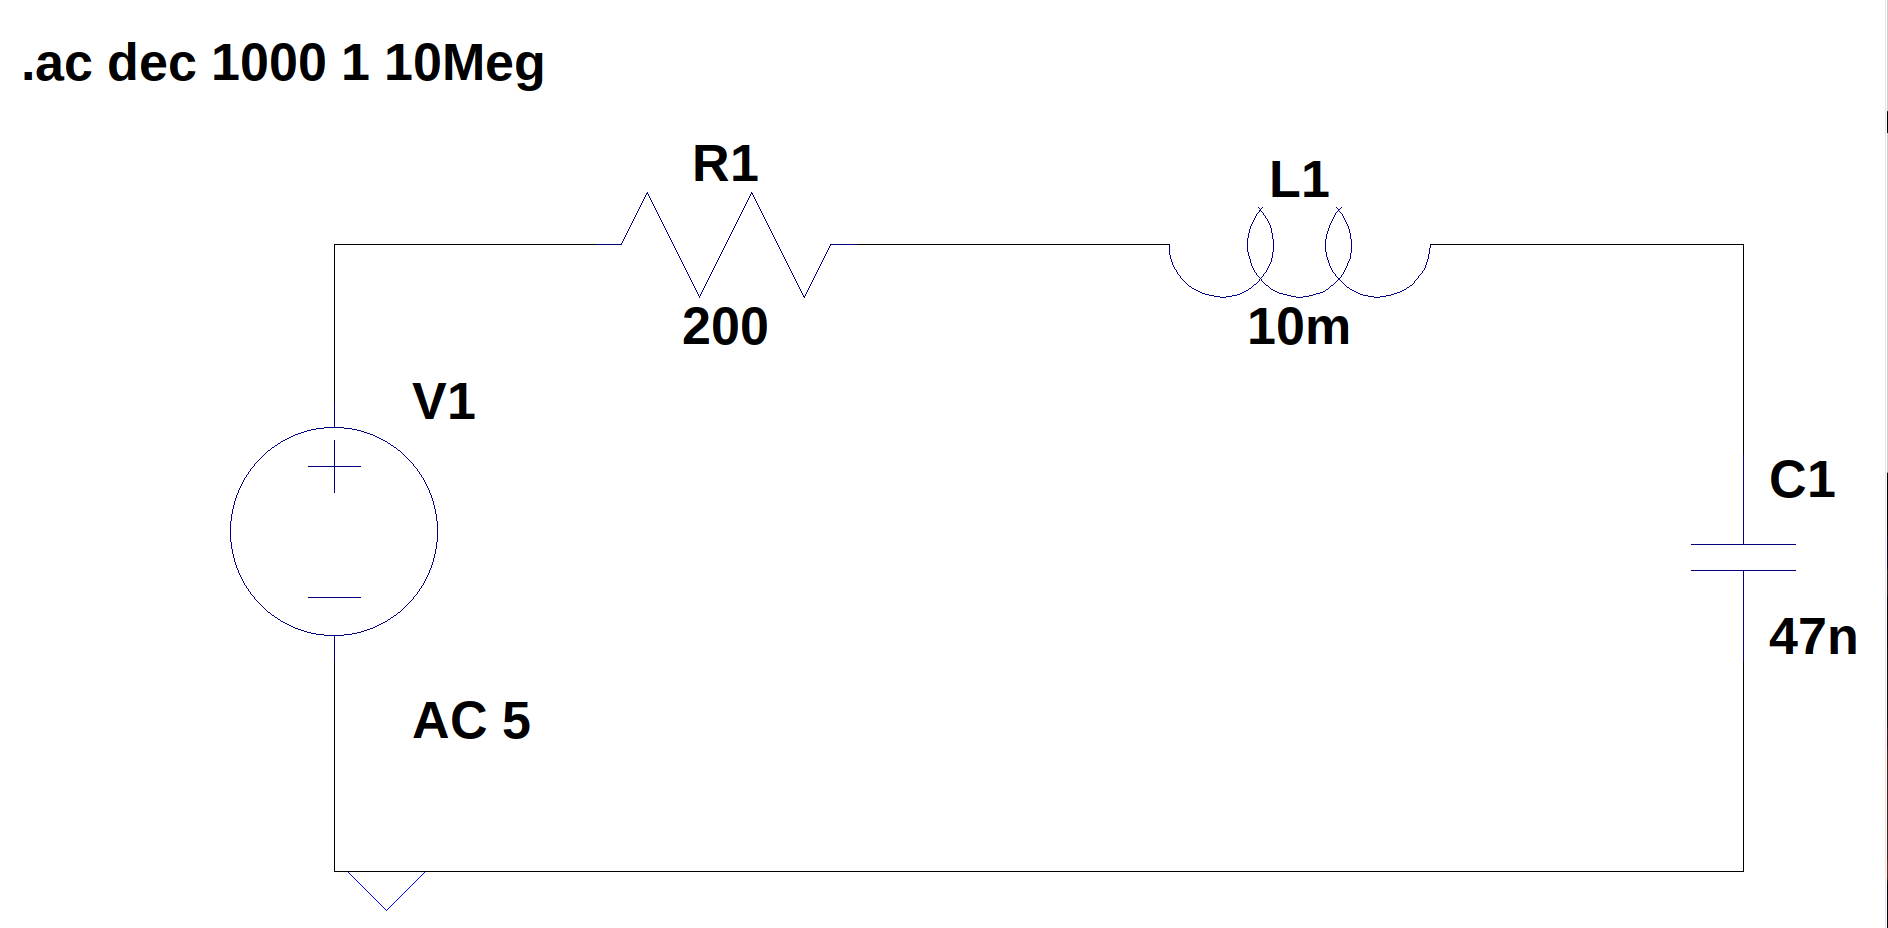
\includegraphics[width=0.5\textwidth]{e6_04}
	\caption{Circuit Four – RLC Bandpass Filter ($R = 200\,\Omega$)}
	\label{fig:circuit4a}
\end{figure}

\noindent \textbf{Measured Values:}
\begin{itemize}
	\item Lower 3dB Point: $5105.05\,\mathrm{Hz}$, Phase: $-30.28^\circ$
	\item Upper 3dB Point: $5597.57\,\mathrm{Hz}$, Phase: $-28.30^\circ$
\end{itemize}

\subsubsection*{Case 2: $R = 2000\,\Omega$ (Overdamped)}
\begin{figure}[H]
	\centering
	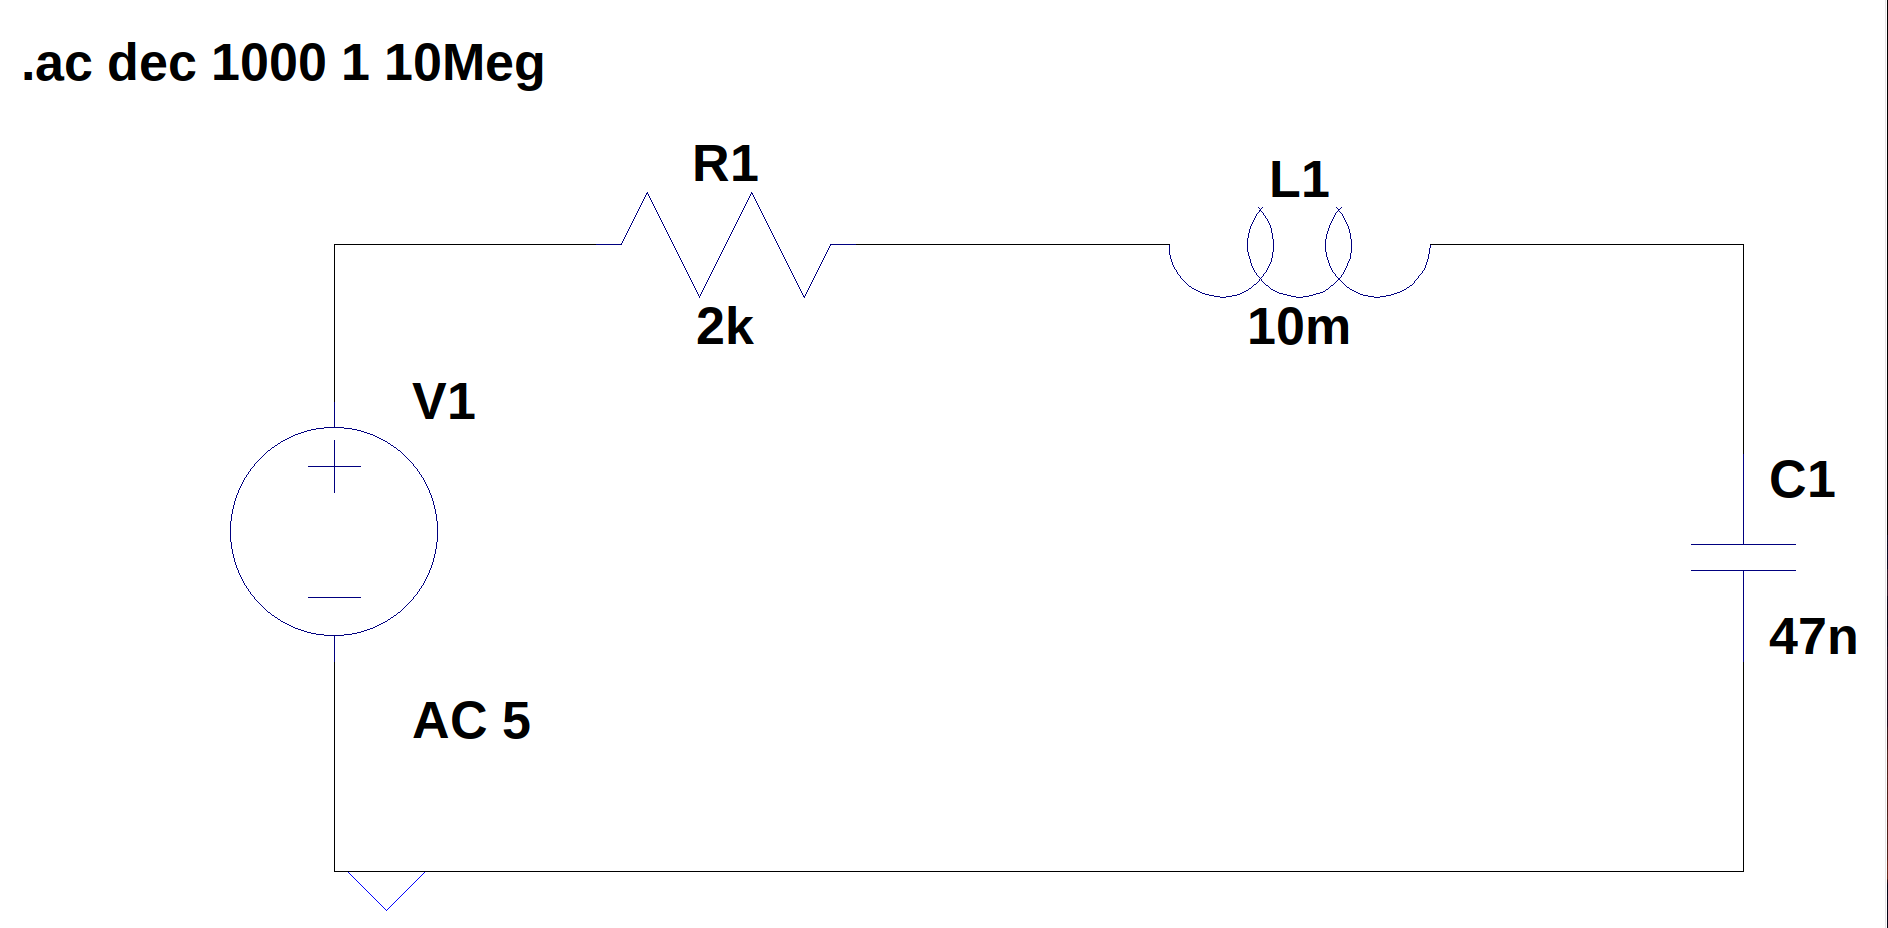
\includegraphics[width=0.5\textwidth]{e6_05}
	\caption{Circuit Four – RLC Low-Pass Behavior ($R = 2000\,\Omega$)}
	\label{fig:circuit4b}
\end{figure}

\noindent In this configuration, the circuit became overdamped. Resonant behavior was suppressed, and the frequency response resembled a second-order low-pass filter.
\section{Results and Discussion}
\subsection{High-Pass Filter Analysis}
Simulation in SPICE following data acquisition was simple. The filter acted as
expected with minimal deviation from the simulated values. See
Table \ref{tab:circuitone}.
\begin{table}[H]
	\centering
	\begin{tabular}{|r|r|r|}
		\hline
		\textbf{Frequency (Hz)} & \textbf{Gain (dB)} & \textbf{Phase ($^\circ$)} \\
		\hline
		1.00                    & -81.680            & 123.927                   \\
		5.99                    & -54.359            & 86.142                    \\
		35.94                   & -41.073            & 86.300                    \\
		215.44                  & -26.350            & 85.221                    \\
		1291.55                 & -11.371            & 70.992                    \\
		\textbf{3569.05}        & \textbf{-4.393}    & \textbf{50.071}           \\
		7742.64                 & -1.522             & 30.026                    \\
		46415.90                & -0.076             & 6.315                     \\
		278256.00               & 0.014              & 1.098                     \\
		10000000.00             & 0.040              & -0.450                    \\
		\hline
	\end{tabular}
	\caption{Scopy Measurements – Circuit 1: RC High-Pass Filter}
	\label{tab:circuitone}
\end{table}

\begin{figure}[H]
	\centering
	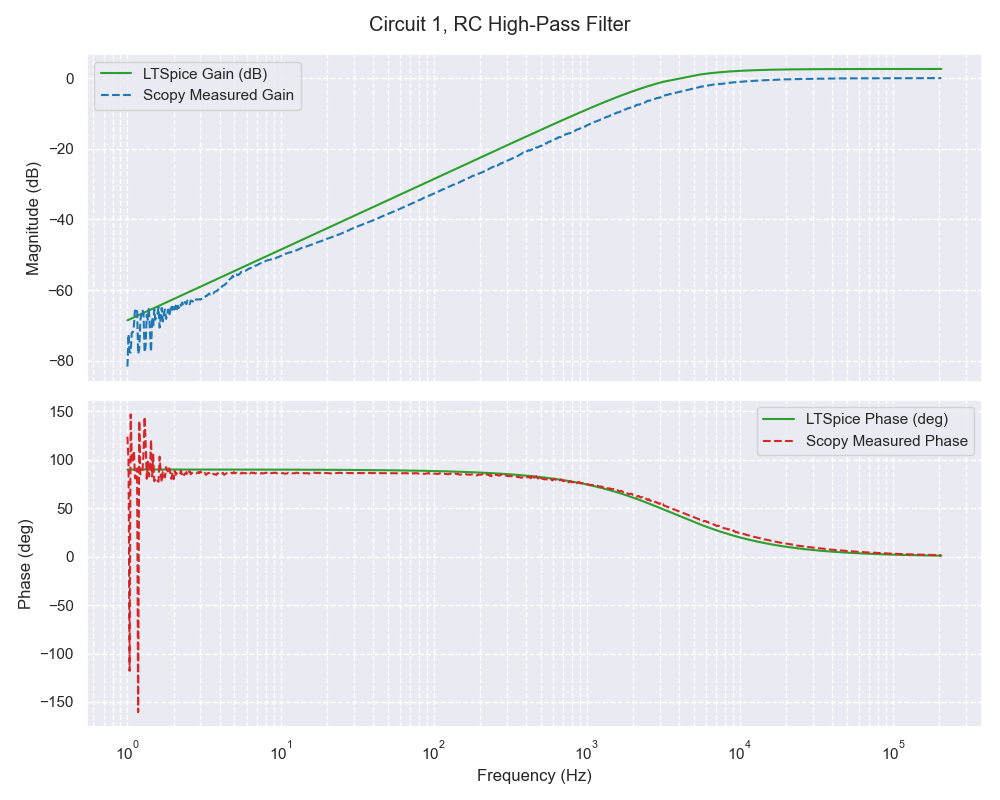
\includegraphics[width=0.75\textwidth]{e6_bode1}
	\caption{Circuit One Results, Resistor Output}
\end{figure}

The Theoretical cutoff frequency calculation for this is \[
	f_c = \frac{\omega_c}{2\pi} = \frac{1}{2\pi RC}.
\]
\[
	f_c = 3617Hz
\]
The experimental results come quite close to those as noted in
Table \ref{tab:circuitone} in bold. The bode plot also shows a phase shift at
higher frequencies closer to $0^\circ$.

\subsection{Low-Pass Filter Analysis}
When the output is taken off the capacitor, however, a completely different
behavior is noted. This acts now as a low pass filter which attenuates higher
frequencies above the cutoff calculation as noted in Table \ref{tab:circuittwo}.

\begin{table}[H]
	\centering
	\begin{tabular}{|r|r|r|}
		\hline
		\textbf{Frequency (Hz)} & \textbf{Gain (dB)} & \textbf{Phase ($^\circ$)} \\
		\hline
		1.00                    & -0.045             & -0.779                    \\
		5.99                    & -0.031             & -0.058                    \\
		35.94                   & -0.036             & -0.487                    \\
		215.44                  & -0.063             & -2.738                    \\
		1291.55                 & -0.507             & -15.575                   \\
		\textbf{3686.10}        & \textbf{-2.466}    & \textbf{-37.314}          \\
		7742.64                 & -6.089             & -56.304                   \\
		46415.90                & -19.171            & -78.441                   \\
		278256.00               & -33.672            & -78.289                   \\
		10000000.00             & -38.133            & 141.555                   \\
		\hline
	\end{tabular}
	\caption{Scopy Measurements – Circuit 2: RC Low-Pass Filter}
	\label{tab:circuittwo}
\end{table}
\begin{figure}[H]
	\centering
	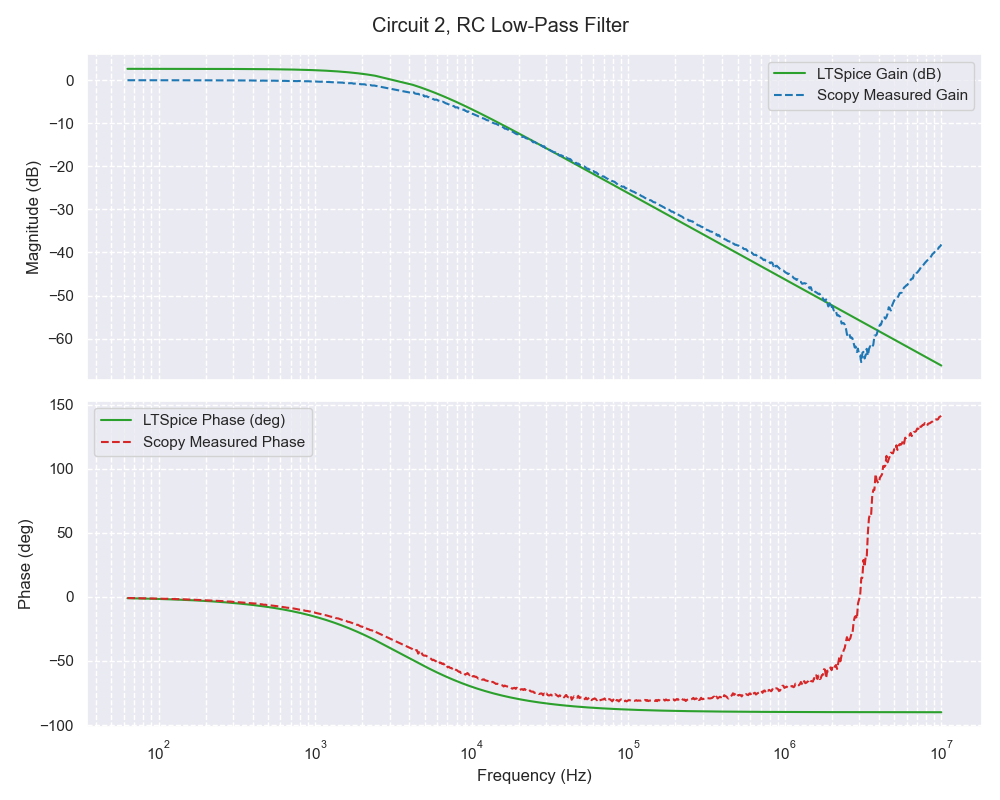
\includegraphics[width=0.75\textwidth]{e6_bode2}
	\caption{Bode Plot Circuit One, Capacitor Output}
	\label{fig:scopycirc2}
\end{figure}

The Theoretical cutoff frequency circuit is the same as the previous,\[
	f_c = \frac{\omega_c}{2\pi} = \frac{1}{2\pi RC}.
\]
\[
	f_c = 3617Hz
\]
Intuitively, the phase plot makes sense for both of these circuits. The
capacitor in the circuit starts by providing a high reactance to the circuit
which as the frequency increases, proportionately decreases to give the
phase response its characteristic shape, although this time it starts at
$0^\circ$ and goes towards $-180^\circ$.

\subsection{Circuit Three: RC Parallel Filter}

The Bode plot in Figure~\ref{fig:scopycircthree} demonstrates strong agreement
between the SPICE simulation and the Scopy measurements for Circuit 3. The
measured cutoff frequency was approximately $f_c = 1377.65\,\mathrm{Hz}$.

\begin{table}[H]
	\centering
	\begin{tabular}{|r|r|r|}
		\hline
		\textbf{Frequency (Hz)} & \textbf{Gain (dB)} & \textbf{Phase ($^\circ$)} \\
		\hline
		1.00                    & -0.072             & -0.738                    \\
		5.99                    & -0.048             & -0.242                    \\
		35.94                   & -0.061             & -1.382                    \\
		215.44                  & -0.156             & -7.839                    \\
		\textbf{1377.65}        & \textbf{-2.385}    & \textbf{-42.622}          \\
		7742.64                 & -14.098            & -101.253                  \\
		46415.90                & -37.471            & -147.796                  \\
		278256.00               & -66.917            & -168.630                  \\
		1668100.00              & -64.770            & 101.918                   \\
		10000000.00             & -40.640            & 150.371                   \\
		\hline
	\end{tabular}
	\caption{Scopy Measurements – Circuit 3: RC Parallel Low-Pass Filter}
\end{table}
\begin{figure}[H]
	\centering
	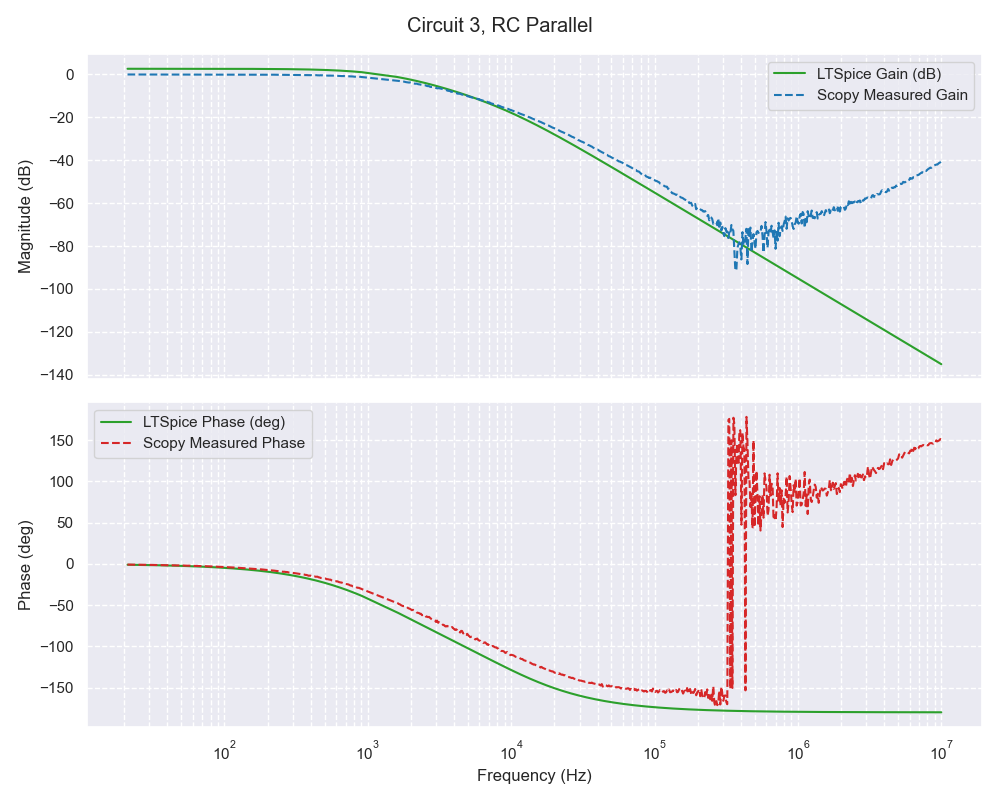
\includegraphics[width=0.75\textwidth]{e6_bode3}
	\caption{Parallel Circuit Response}
	\label{fig:scopycircthree}
\end{figure}

To quantify the stopband behavior, the gain slope was computed between $7.7$ kHz
and $46.4$ kHz.
\[
	\text{Slope} = \frac{-37.471 - (-14.098)}{\log_{10}(46415.90) - \log_{10}(7742.64)} \approx -30.08\,\mathrm{dB/decade}
\]
This suggests second-order behavior, since the slope is steeper than that of a first-order filter but not as sharp as the ideal $-40\,\mathrm{dB/decade}$. In contrast, the stopband slope for Circuit 2 (RC low-pass) was calculated as:
\[
	\text{Slope}_{\text{Circuit 2}} = \frac{-19.171 - (-6.089)}{\log_{10}(46415.90) - \log_{10}(7742.64)} \approx -16.83\,\mathrm{dB/decade}
\]

This value aligns well with the expected $-20\,\mathrm{dB/decade}$ slope of a first-order filter. Thus, the sharper slope observed in Circuit 3 confirms its higher-order behavior.

\subsection{RLC Bandpass Filter}

The RLC bandpass filter implemented with $R = 200\,\Omega$ demonstrated classic underdamped behavior, exhibiting a distinct resonance peak between 5\,kHz and 6\,kHz. From the measured data in Table~\ref{tab:rlc_bandpass}, the peak gain occurs near $f_0 = 5607.23\,\mathrm{Hz}$ with a gain of $4.286\,\mathrm{dB}$. The phase sharply transitions through $-90^\circ$, a hallmark of second-order bandpass filters.

\begin{table}[H]
	\centering
	\caption{Scopy Measurements – Circuit Four, RLC Bandpass Filter ($R=200\,\Omega$)}
	\label{tab:rlc_bandpass}
	\begin{tabular}{|r|r|r|}
		\hline
		\textbf{Frequency (Hz)} & \textbf{Gain (dB)} & \textbf{Phase ($^\circ$)} \\
		\hline
		1.00                    & 18.009             & 1.113                     \\
		5.99                    & -0.016             & -0.019                    \\
		35.94                   & -0.016             & -0.138                    \\
		215.44                  & -0.017             & -0.797                    \\
		1291.55                 & 0.174              & -5.155                    \\
		\textbf{5089.87}        & \textbf{3.675}     & \textbf{-33.948}          \\
		\textbf{5607.23}        & \textbf{4.286}     & \textbf{-40.791}          \\
		7742.64                 & 4.358              & -95.247                   \\
		46415.90                & -28.705            & -168.845                  \\
		278256.00               & -64.036            & -175.566                  \\
		\hline
	\end{tabular}
\end{table}

\begin{figure}[H]
	\centering
	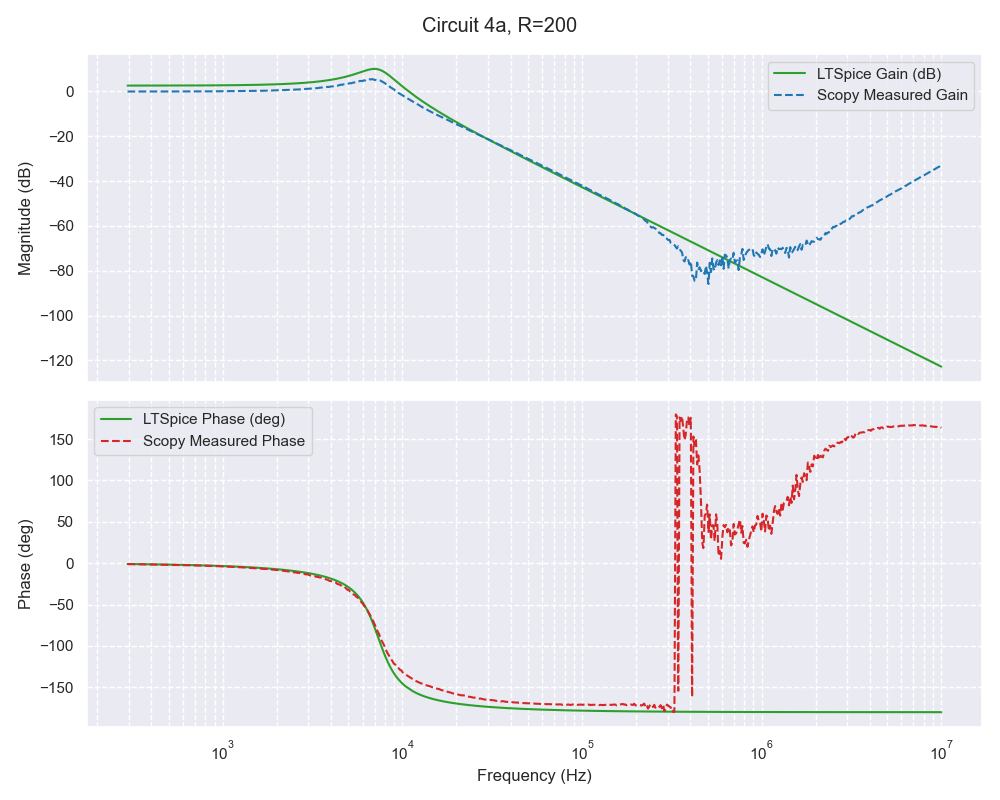
\includegraphics[width=0.5\textwidth]{e6_bode4}
	\caption{Measured and Simulated Bode Plot – Circuit Four ($R = 200\,\Omega$)}
\end{figure}

\begin{figure}[H]
	\centering
	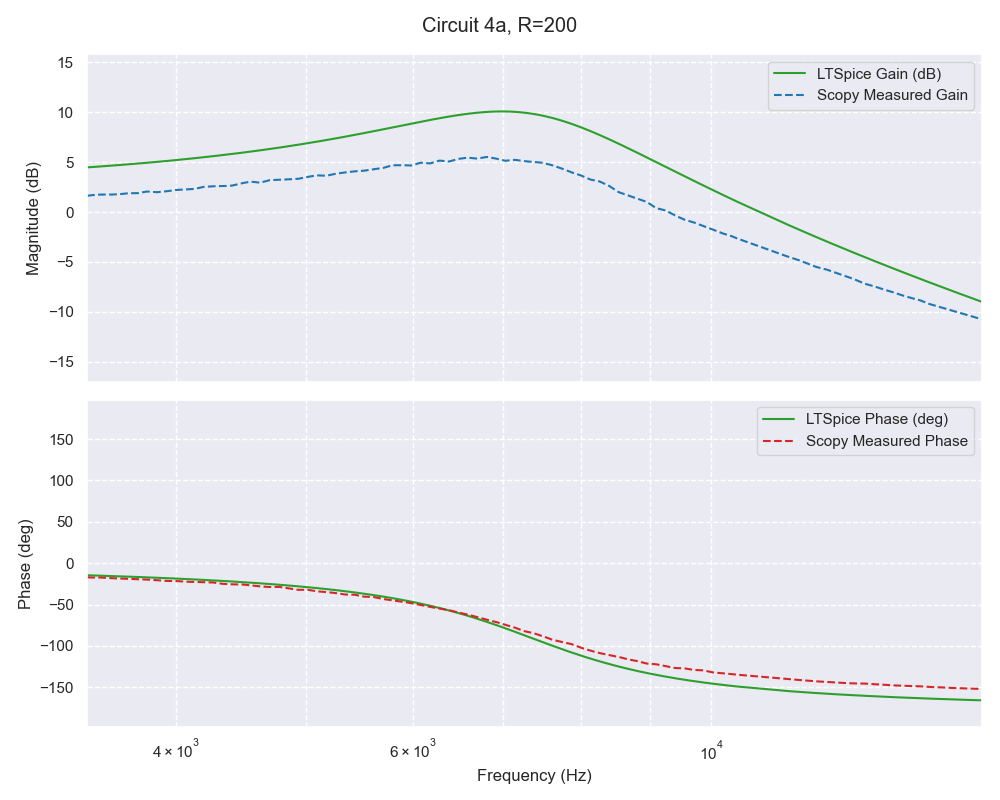
\includegraphics[width=0.8\textwidth]{e6_bandbode}
	\caption{Zoomed View of Resonance Peak – Circuit Four ($R = 200\,\Omega$)}
\end{figure}

The agreement between SPICE and Scopy data confirms resonance in this underdamped case. The amplitude peak and steep phase transition indicate a high quality factor \( Q \), consistent with the lower resistance value. The bandwidth can be estimated from the 3\,dB drop-off points around the peak, enabling further computation of the selectivity and damping characteristics.

\subsection{Overdamped Case}

When the resistance in the RLC circuit was increased to $2000\,\Omega$, the system became overdamped. The frequency response showed no resonance peak and instead exhibited a gradual, monotonic roll-off.

\begin{figure}[H]
	\centering
	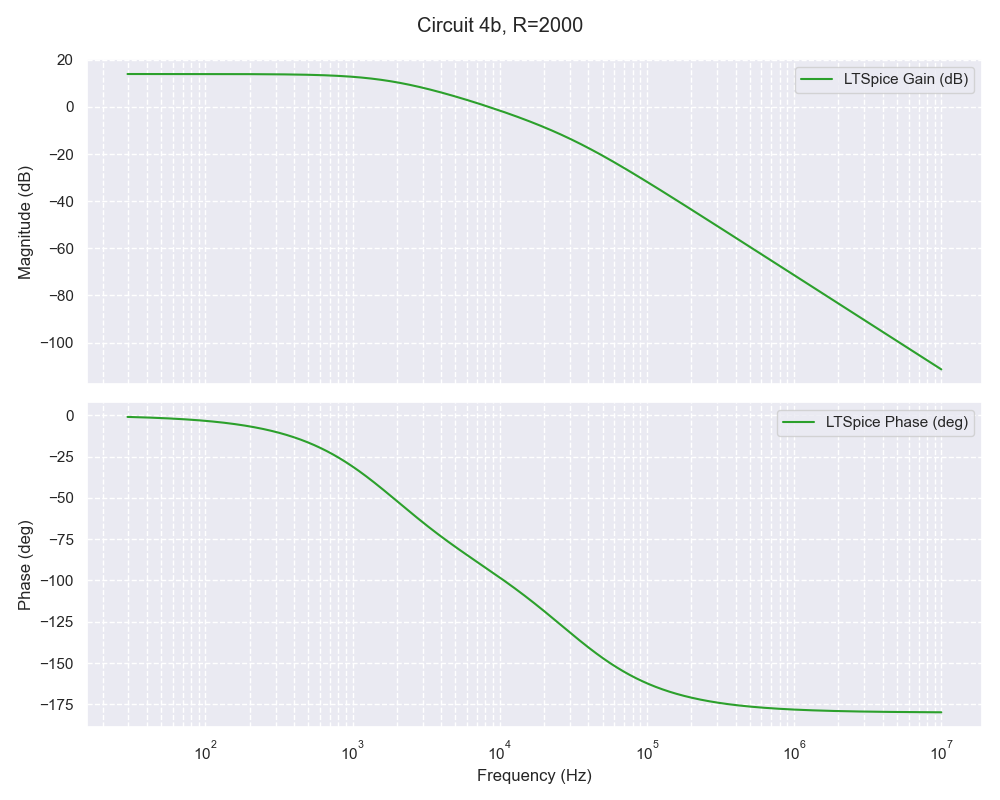
\includegraphics[width=\textwidth]{e6_bode5}
	\caption{SPICE Bode Plot – Circuit Four, RLC Low-Pass Filter ($R = 2000\,\Omega$)}
	\label{fig:rlc_lp}
\end{figure}

This behavior illustrates the direct impact of resistance on the damping ratio and quality factor \( Q \). As $R$ increases, the energy in the circuit is dissipated more rapidly, reducing selectivity and flattening the response. The phase shift also smooths out across frequencies, resembling a second-order low-pass filter.

\section{Conclusion}

Across all circuits tested, measured amplitude and phase responses closely aligned with LTSpice simulations, validating theoretical predictions and highlighting practical circuit behavior.

\paragraph{Summary of Filter Types}
\begin{itemize}
	\item \textbf{Circuit One (Resistor Output)}: First-order high-pass filter
	\item \textbf{Circuit Two (Capacitor Output)}: First-order low-pass filter
	\item \textbf{Circuit Three (Parallel RC)}: Second-order low-pass filter
	\item \textbf{Circuit Four ($R = 200\,\Omega$)}: Underdamped bandpass filter
	\item \textbf{Circuit Four ($R = 2000\,\Omega$)}: Overdamped second-order low-pass filter
\end{itemize}

This lab demonstrated the significance of passive components in shaping signal
behavior across the frequency spectrum. The comparison of experimental and
simulated data confirms the reliability of both analytical methods and software
tools like SPICE. These foundations are crucial for future work in analog signal processing, communication electronics, and filter design.
\end{document}
% vim: set ft=tex tw=80 ts=2 sts=2 sw=2 noet spell:
